\documentclass[11pt,letterpaper]{article}
\usepackage[utf8]{inputenc}
\usepackage{graphicx}
\usepackage{caption}
\usepackage{subcaption}
\author{Michael D. Brothers}
\title{Homework 7}
\begin{document}

\section{Problem 1.1.1}

\begin{figure}[!tbh]
    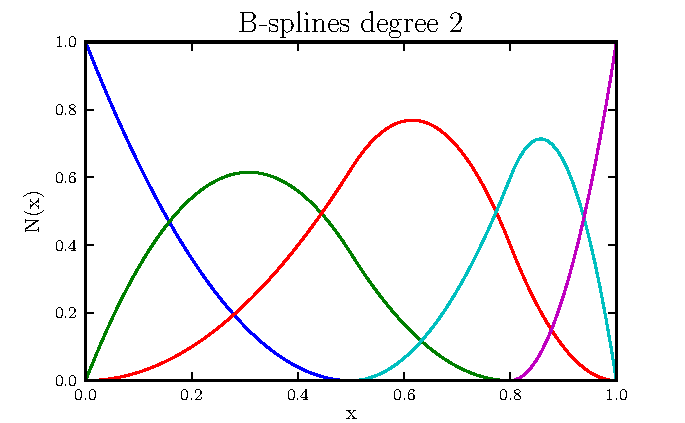
\includegraphics[width=\textwidth]{problem_1_1_1.pdf}
    \caption{\textbf{Zeros}: 
    The values of the basis functions are zero where they are defined to be zero, according to their Cox-DeBoor recursive definition in terms of box functions. 
    These box functions select over what intervals defined by the knot vector evaluate to nonzero for the given basis function. 
    The box functions can be determined easily by using a tree diagram created by inspecting the Cox-DeBoor formula for the desired basis function as was done in the handwritten component to this assignment.\\
    \textbf{Smoothness}:
    N1 is smooth from knot 1 to knot 2. N2 is smooth from knot 1 to knot 3. N3 is smooth from knot 1 to knot 4. N4 is smooth from knot 2 to knot 4. N5 is smooth from knot 3 to knot 4. 
    I say smooth since these functions are just polynomials over the intervals for which they are nonzero.}
    \label{fig1:label:a}

\end{figure}

\section{Problem 1.2.1}

\begin{figure}[!tbh]
\centering
 \begin{tabular}{rrrrrr}
\hline
  Num & u=0.0 &   u=0.25 &   u=0.5 &    u=0.75 &   u=1.0 \\
\hline
  N1 &     1 &  0.25    &   0     & 0         &       0 \\
  N2 &     0 &  0.59375 &   0.375 & 0.0104167 &       0 \\
  N3 &     0 &  0.15625 &   0.625 & 0.572917  &       0 \\
  N4 &      0 &  0       &   0     & 0.416667  &       0 \\
  N5 &     0 &  0       &   0     & 0         &       1 \\
\hline
\end{tabular}
\caption{Basis function evaluations for original knot vector.}
\label{tab1}
\end{figure}

\begin{figure}[!tbh]
\centering
\begin{tabular}{rrrrrr}
\hline
   Num & u=0.0 &   u=0.25 &   u=0.5 &    u=0.75 &   u=1.0 \\
\hline
   N1&    1 &     0.25 &       0 & 0         &       0 \\
   N2&    0 &     0.5  &       0 & 0         &       0 \\
   N3&    0 &     0.25 &       1 & 0.0277778 &       0 \\
   N4&    0 &     0    &       0 & 0.555556  &       0 \\
   N5&    0 &     0    &       0 & 0.416667  &       0 \\
   N6&    0 &     0    &       0 & 0         &       1 \\
\hline
\end{tabular}
\caption{Basis function evaluations for part a.}
\label{tab2}
\end{figure}


\begin{figure}[!tbh]
\centering
\begin{tabular}{rrrrrr}
\hline
  Num &  u=0.0 &   u=0.25 &   u=0.5 &     u=0.75 &   u=1.0 \\
\hline
  N1 &     1 & 0.125    &   0     & 0          &       0 \\
  N2 &     0 & 0.375    &   0     & 0          &       0 \\
  N3&     0 & 0.421875 &   0.375 & 0.00173611 &       0 \\
  N4&      0 & 0.078125 &   0.625 & 0.072338   &       0 \\
  N5&     0 & 0        &   0     & 0.578704   &       0 \\
  N6&     0 & 0        &   0     & 0.347222   &       0 \\
  N7&     0 & 0        &   0     & 0          &       0 \\
  N8&     0 & 0        &   0     & 0          &       1 \\
\hline
\end{tabular}
\caption{Basis function evaluations for part b.}
\label{tab3}
\end{figure}

\begin{figure}[!tbh]
\centering
\begin{tabular}{rrrrrr}
\hline
   Num & u=0.0 &    u=0.25 &   u=0.5 &    u=0.75 &   u=1.0 \\
\hline
   N1&    1 & 0.0277778 &     0   & 0         &       0 \\
   N2&    0 & 0.555556  &     0   & 0         &       0 \\
     N3&  0 & 0.416667  &     0.6 & 0.0166667 &       0 \\
    N4&   0 & 0         &     0.4 & 0.566667  &       0 \\
    N5&   0 & 0         &     0   & 0.416667  &       0 \\
    N6&   0 & 0         &     0   & 0         &       1 \\
\hline
\end{tabular}
\caption{Basis function evaluations for part c.}
\label{tab4}
\end{figure}

\begin{figure}[!tbh]
\centering
\begin{tabular}{rrrrr}
\hline
   u=0.0 &   u=0.25 &   u=0.5 &   u=0.75 &   u=1.0 \\
\hline
      50 &  140.625 &   212.5 &  290.625 &     450 \\
      50 &  109.375 &    87.5 &  134.375 &     250 \\
\hline
\end{tabular}
\caption{Curve evaluations for original knot vector.}
\label{tab5}
\end{figure}

\begin{figure}[!tbh]
\centering
\begin{tabular}{rrrrr}
\hline
   u=0.0 &   u=0.25 &   u=0.5 &   u=0.75 &   u=1.0 \\
\hline
      50 &  141.875 &   217.5 &  290.764 &     450 \\
      50 &  109.375 &    87.5 &  134.375 &     250 \\
\hline
\end{tabular}
\caption{Curve evaluations for part a.}
\label{tab6}
\end{figure}

\begin{figure}[!tbh]
\centering
\begin{tabular}{rrrrr}
\hline
   u=0.0 &   u=0.25 &   u=0.5 &   u=0.75 &   u=1.0 \\
\hline
      50 &  140.859 & 212.875 &  290.777 &     450 \\
      50 &  109.391 &  87.125 &  134.223 &     250 \\
\hline
\end{tabular}
\caption{Curve evaluations for part b.}
\label{tab7}
\end{figure}

\begin{figure}[!tbh]
\centering
\begin{tabular}{rrrrr}
\hline
   u=0.0 &   u=0.25 &   u=0.5 &   u=0.75 &   u=1.0 \\
\hline
      50 &  140.625 &   212.5 &  290.625 &     450 \\
      50 &  109.375 &    87.5 &  134.375 &     250 \\
\hline
\end{tabular}
\caption{Curve evaluations for part c.}
\label{tab8}
\end{figure}

It was expected that refinement by any procedure including knot insertion, degree elevation, or increasing multiplicity at a single knot would leave the geometry of the curve being represented unaltered.
The control points for part b were taken from the example widget from the link provided in the homework. Largely the geometry was not disrupted, since the curve evaluations varried little from case to case in Figs. \ref{tab5}, \ref{tab6}, \ref{tab7} and \ref{tab8}.
The discrepancies are confusing, and I think they come from inaccuracies in my evaluation procedure, since if the procedure was completely wrong I would expect bigger differences. \\

Since the control point interpolates at the endpoints of the curve, it is no wonder that the evaluations match perfectly at the endpoints.










\end{document}
